\documentclass[9pt,twoside,lineno]{pnas-new}
% Use the lineno option to display guide line numbers if required.

\templatetype{pnassupportinginfo}

% Math
\def\P{\mathbb{P}}
\def\cor{\mathrm{cor}}
\def\Quantile{\mathrm{Quantile}}
\def\logit{\mathrm{logit}}
\def\dist{\mathrm{dist}}
\def\WIS{\mathrm{WIS}}
\def\AUC{\mathrm{AUC}}
\newcommand{\indicator}[1]{\mathbf{1}\left(#1\right)}

% Figures and tables
\usepackage{xurl}
\usepackage{microtype}
\usepackage{booktabs}
\usepackage{caption}
\usepackage{subcaption}
\usepackage{xcolor}
\newcommand{\attn}[1]{\textcolor{red}{[ATTN: #1]}}

\makeatletter 
\renewcommand\@biblabel[1]{#1} 
\makeatother

% indicators
\newcommand{\chngcli}{CHNG-CLI}
\newcommand{\chngcov}{CHNG-COVID}
\newcommand{\dv}{DV-CLI}
\newcommand{\ar}{AR}
\newcommand{\fb}{CTIS-CLI-in-community}
\newcommand{\gs}{Google-AA}


\providecommand{\tightlist}{%
  \setlength{\itemsep}{0pt}\setlength{\parskip}{0pt}}

$for(header-includes)$
$header-includes$
$endfor$

\title{Your main manuscript title}
\author{Author1, Author2 and Author3 (complete author list)}
\correspondingauthor{Corresponding Author name.\\E-mail: author.two@email.com}

\begin{document}

%% Comment out or remove this line before generating final copy for submission; this will also remove the warning re: "Consecutive odd pages found".
\instructionspage  

\maketitle

%% Adds the main heading for the SI text. Comment out this line if you do not have any supporting information text.
\SItext


\section*{PNAS Template material, to be removed}

\subsection*{Subhead}
Type or paste text here. This should be additional explanatory text such as an extended technical description of results, full details of mathematical models, etc.   

\section*{Heading}
\subsection*{Subhead}
Type or paste text here. You may break this section up into subheads as needed (e.g., one section on ``Materials'' and one on ``Methods'').

\subsection*{Materials}
Add a materials subsection if you need to.

\subsection*{Methods}
Add a methods subsection if you need to.


%%% Each figure should be on its own page
\begin{figure}
\centering
\includegraphics[width=\textwidth]{example-image}
\caption{First figure}
\end{figure}

\begin{figure}
\centering
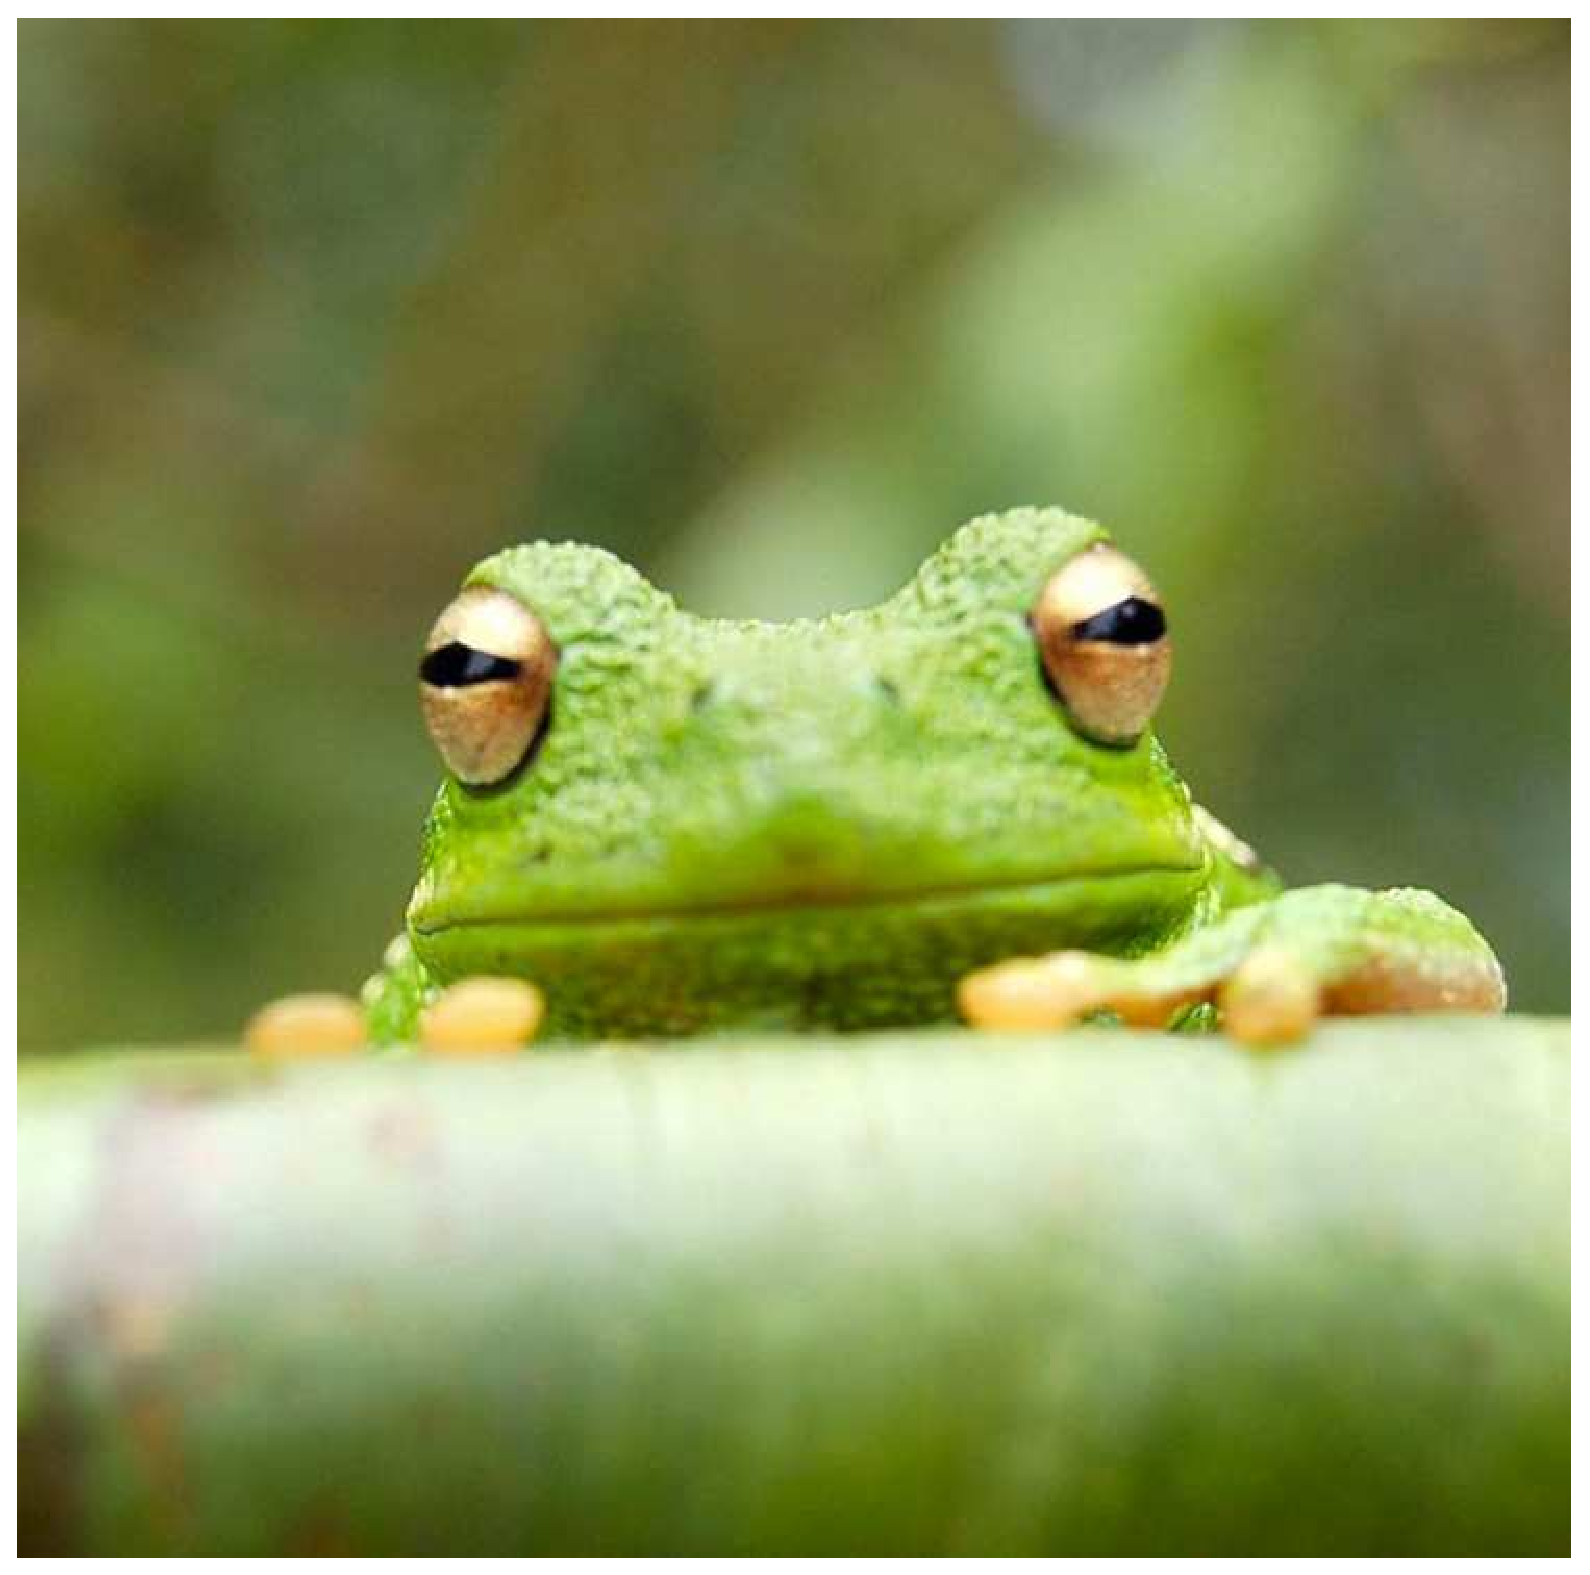
\includegraphics[width=\textwidth]{pnas-materials/frog}
\caption{Second figure}
\end{figure}

\begin{table}\centering
\caption{This is a table}

\begin{tabular}{lrrr}
Species & CBS & CV & G3 \\
\midrule
1. Acetaldehyde & 0.0 & 0.0 & 0.0 \\
2. Vinyl alcohol & 9.1 & 9.6 & 13.5 \\
3. Hydroxyethylidene & 50.8 & 51.2 & 54.0\\
\bottomrule
\end{tabular}
\end{table}


\clearpage

$body$



%%% Add this line AFTER all your figures and tables
\FloatBarrier

\movie{Type legend for the movie here.}

\movie{Type legend for the other movie here. Adding longer text to show what happens, to decide on alignment and/or indentations.}

\movie{A third movie, just for kicks.}

\dataset{dataset_one.txt}{Type or paste legend here.}

\dataset{dataset_two.txt}{Type or paste legend here. Adding longer text to show what happens, to decide on alignment and/or indentations for multi-line or paragraph captions.}


\bibliography{$for(bibliography)$$bibliography$$sep$,$endfor$}

\end{document}